%% Template for Master thesis
%% ===========================
%%
%% You need at least KomaScript v3.0.0,
%% e.g. available in Texlive 2009
\documentclass  [
  paper    = a4,
  BCOR     = 10mm,
  twoside,
  fontsize = 12pt,
  fleqn,
  toc      = bibnumbered,
  toc      = listofnumbered,
  numbers  = noendperiod,
  headings = normal,
  listof   = leveldown,
  version  = 3.03
]                                       {scrreprt}

% used pagages
\usepackage     [utf8]                  {inputenc}
\usepackage     [T1]                    {fontenc}
\usepackage                             {color}
\usepackage                             {amsmath}
\usepackage                             {graphicx}
\usepackage     [english]               {babel}
\usepackage                             {natbib}
\usepackage                             {hyperref}

% links
\definecolor{darkblue}{rgb}{0.0,0.0,0.4}
\definecolor{darkgreen}{rgb}{0.0,0.4,0.0}
\hypersetup{
    colorlinks,
    linkcolor=black,
    citecolor=darkgreen,
    urlcolor=darkblue
}

\begin{document}
  %% title pages similar to providet template instead of maketitle
  %% Titelseiten ähnlich zum Layout des Formulars von der
%% Fakultät für Physik und Astronomie
%%
%% Weitere Infos:
%% http://www.physik.uni-heidelberg.de/aktuelles/studium/
%% (PDF link: ...studium/download/145/Vorlage_Diplomarbeit_Formular.pdf)

%% Titelintro
\thispagestyle{empty}
\begin{center}
  \renewcommand{\baselinestretch}{2.00}
  \Large\sffamily
  Fakult\"{a}t f\"{u}r Physik und Astronomie\\
  \large
  Ruprecht-Karls-Universit\"{a}t Heidelberg
  \par\vfill\normalfont
  Masterarbeit\\
  Im Studiengang Physik\\
  vorgelegt von\\
  Martin Huber\\
  geboren in Frankenthal (Pfalz)\\
  2019\\
\end{center}
\newpage

%% Titelseite
\thispagestyle{empty}
\begin{center}
  \renewcommand{\baselinestretch}{2.00}
  \Large\bfseries\sffamily
    Implementierung und Fusion von \\
    modellprädiktiver Regelung mit \\
    neuronalen Netzwerken zur \\ 
    autonomen Navigation von humanoiden Robotern
  \par
  \vfill
  \large\normalfont
  Die Masterarbeit wurde von Martin Huber\\
  ausgeführt am\\
  Institut für Optimierung, Robotik und Biomechanik\\
  unter der Betreuung von\\
  Frau Prof. Katja Mombaur
  %% Bei externen Masterarbeiten hier noch den zweiten Betreuer einfügen
  %% und den vspace in Z. 45 entsprechend reduzieren
\end{center}\par
\vspace{5\baselineskip}

% Zeilenabstand zurücksetzen
\renewcommand{\baselinestretch}{1.00}\normalsize % select either german
  \include{chapters/00_titletitlepages-eng} % or english title page
  %% Abstract page
%% =============
%%
%% Content of abstract pages has been put into seperate pages to simplify
%% word counting. Use e.g. the unix command
%%   wc abstract-ger.tex
%% or
%%   wc abstract-eng.tex
%% to get the number of words contained in these files.
\thispagestyle{empty}
\begin{center}
  \begin{minipage}[c][0.48\textheight][b]{0.9\textwidth}
    \small
    \textbf{
      Verhaltensklonung zur autonomen Navigation humanoider Roboter mit Nichlinearer Modellprädiktiver Regelung:
    }\par
    \vspace{\baselineskip}
    In dieser Arbeit erkunden wir die Möglichkeiten der Verhaltensklonung zur autonomen Navigation humanoider Roboter durch bloße Bilder. Hierfür wird eine nichtlineare, Modellprädiktive Regelung, die es ermöglicht, stabile Lauftrajektorien in Echtzeit zu erzeugen, implementiert und evaluiert. Es wird demonstriert, dass minimale Veränderung in der Bildverarbeitung genügen, um vielseitige Bewegungsstrategien in vielfältigen dynamischen und statischen Umgebungen zu erlernen. Diese Einfachheit der Lösung wird als passende Ergänzung zur Meidung von Konvexen Hindernissen identifiziert, welche durch Randbedingungen die Lösungen der nichtlinearen Modellprädiktiven Regelung einschränken. Alle Experimente werden an Heicub, einer Variente des iCub, durchgeführt, welcher speziell für Optimalsteuerung in der Fortbewegung am Istituto Italiano di Tecnologiia in Genove entwickelt wurde. Die Auswertung von Stabilitätskriterien zeigt weiterhin, dass ein menschlicher Kontrolleur, einem künstlichen Agenten gegenüber, nicht überlegen ist. Um die präsentierte Methode schließlich auf tauschende Aufgaben zu erweitern, vereinfachen wir die wechselnden Umgebungen auf ein gut gelöstes Klassifizierungsproblem.
  \end{minipage}\par
  \vfill
  \begin{minipage}[c][0.48\textheight][b]{0.9\textwidth}
    \small
    \textbf{
      Behavioral Cloning for Autonomous Navigation of Humanoid Robots with Nonlinear Model Predictive Control:
    }\par
    \vspace{\baselineskip}
    In this work, we investigate the capabilities of behavioral cloning for autonomous navigation of humanoid robots from raw image input. Therefore, a nonlinear model predictive control that allows for real-time generation of stable walking trajectories is implemented and evaluated. It is demonstrated that minor modifications in the vision pipeline are sufficient for the learning of versatile motion strategies in various dynamic and static environments. This simplicity is identified as a well-suited addition to the avoidance of convex obstacles, which are represented by constraints to the solution of the implemented nonlinear model predictive control. All of the experiments are carried out on Heicub, a descendant of the iCub, which was specially designed for optimal control in locomotion at the Istituto Italiano di Tecnologia in Genova. The evaluation of balance criteria further reveals that there is no superiority of a human controller over an artificial agent. Finally, we investigate on reinforcement learning methods to replace the behavioral cloning by self-taught policies.

  \end{minipage}
\end{center}


  \tableofcontents
  
  %% chapters
  \chapter{Introduction}
  % humanoids (icub, others), problem statement, research aim and objectives
    
  \chapter{State of the Art}
  \label{sec::2_sota}
  % contributions
    
  \chapter{Background}
  To generate dynamically balanced walking trajectories for humanoid robots and to let them navigate the environment autonomously, there are several posed challenges that we need to cover. As the logical starting point, in section \ref{sec::31_hm} - Humanoid Walking, we want to address the real time generation of walking trajectories for humanoid robots first, and then think of ways to replace the human user by an artificial agent in the control loop. As discussed in section \ref{sec::2_sota} - State of The Art, there are several ways to achieve this, but of particular interest to us are novel methods that evolved from the toolbox of machine learning techniques. Center to these new methods will be neural nets that we will try to train on solving the task of autonomous navigation in different ways, as shown in section \ref{sec::32_ml} - Machine Learning.
\begin{figure}[h]
	\centering
	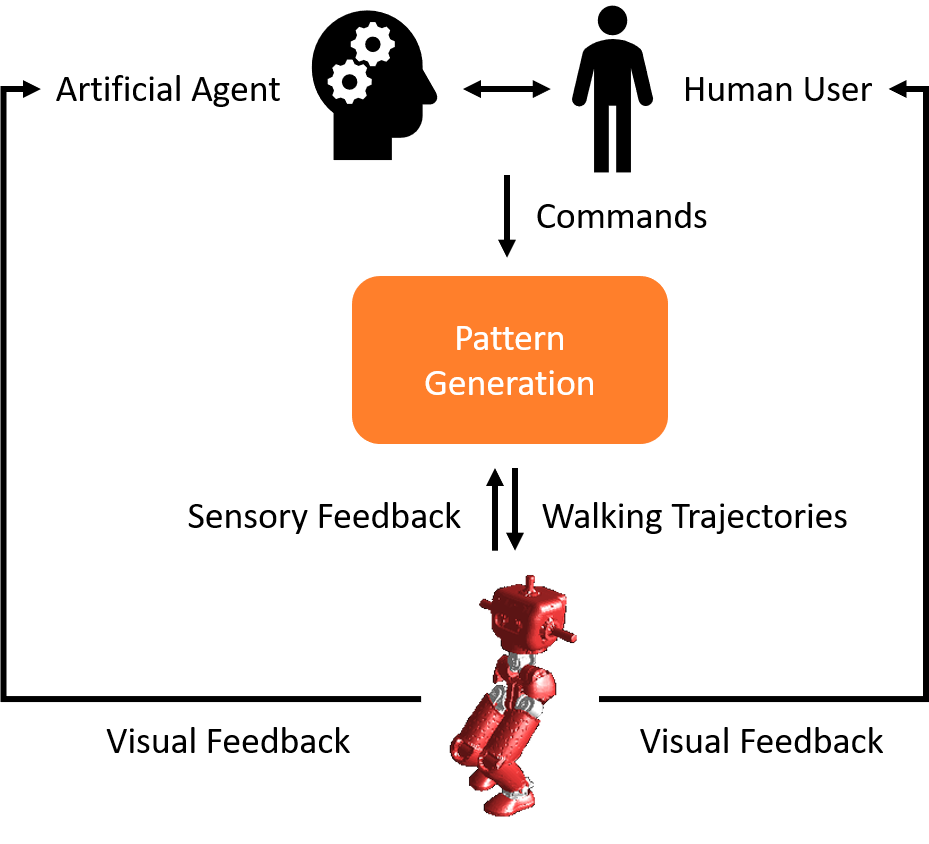
\includegraphics[scale=.5]{chapters/03_background/img/control_loop.png}
	\caption{\label{fig::3_cl} Proposed control loop to navigate the robot with either a human user or an artificial agent.}
\end{figure}   % introduction to background
  \section{Humanoid Walking}
  \label{sec::31_hm}
  \subsection{Zero Moment Point}
\label{sec::311_zmp}
  % zero moment point
  \subsection{Linear Inverted Pendulum}
  % linear inverted pendulum
  \subsection{Nonlinear Model Predictive Control}
 % nonlinear model predictive control
  \subsection{Interpolating Trajectories}
   % interpolation
  \subsection{Kinematics}
   % kinematics
  
  \section{Machine Learning}  
  \label{sec::32_ml}
  \subsection{Behavioral Cloning}
   % behavioral cloning
  \subsection{Reinforcement Learning}
   % reinforcement learning
  \subsection{Image Processing}
   % image processing
   
  \chapter{Methods}
  \section{Software}
  %\input{chapters/04_methods/01_eig}     % eigen
  %\input{chapters/04_methods/02_qp}      % qpoases
  %\input{chapters/04_methods/03_rbdl}    % rbdl
  %\input{chapters/04_methods/04_yarp}    % yarp
  %\input{chapters/04_methods/05_pyt}     % pytorch
  %\input{chapters/04_methods/06_cv}      % opencv
  
  \section{Implementation}  
   
  \chapter{Experiments}
  
  \section{User Controlled Walking}
  
  \section{Autonomous Walking}

  \chapter{Conclusion}

  \part{Appendix}
  \begin{appendix}
    \chapter{Lists}
    \listoffigures
    \listoftables
    \bibliographystyle{plain}
    \bibliography{chapters/07_appendix/references}
    \citestyle{egu}
    \bibliographystyle{plainnat}
    \setlength{\parindent}{0em}

Erkl\"{a}rung:\par
\vspace{3\baselineskip}
Ich versichere, dass ich diese Arbeit selbstst\"{a}ndig verfasst habe und keine
anderen als die angegebenen Quellen und Hilfsmittel benutzt habe.\par
\vspace{5\baselineskip}
Heidelberg, den (Datum)\hspace{3cm}\dotfill

  \end{appendix}
\end{document}
